\Chapter{A MySQL Connector}

\Section{Ismertető}
A MySQL Connector egy MySQL alapú driver JDBC, ODBC, és .NET rendszerek számára. Lehetővé teszi, hogy a fejlesztők adatbázis alkalmazásokat írjanak a támogatott nyelveken. Ezen kívül egy natív C könyvtár teszi lehetővé, hogy a MySQL-t közvetlenül beágyazhassák az alkalmazásaikba.
MySQL által fejlesztett driver -ek:
ADO.NET, ODBC, JDBC, Node.js, Python, C++, C és C API a a klienshez. 
A MySQL közösség által fejlesztetek:
PHP, Perl, Ruby, C+ Wrapper.

*https://www.mysql.com/products/connector/

\Section{A Connector/C++ használata}

Az alábbi weboldalról letöltött állományokat használtam:
https://dev.mysql.com/downloads/connector/cpp/
\begin{itemize}
\item Linux - Generic
\item All
\item Linux - Generic (glibc 2.12) (x86, 64-bit), Compressed TAR Archive
\end{itemize}

Letöltés után kicsomagoljuk. A tartalma egy include és egy lib64 mappa. Az include mappa tartalmát a usr/include könyvtárba másoljuk, a lib64 -ét pedig az usr/lib64 mappába.

Ezután szükség lesz egy külön felhasználóra amellyel a program csatlakozni fog a szerverünkre. Ezt megtehetjük a Workbench alkalmazásban.
\begin{python}
CREATE USER 'newuser'@'localhost' IDENTIFIED BY 'password';
\end{python}

\Section{Első program}

Hozzunk létre egy \texttt{connectortest.cpp} nevű fájlt.
\begin{cpp}
#include <iostream>
#include <stdlib.h>
#include "mysql_connection.h"
#include <cppconn/driver.h>
#include <cppconn/exception.h>
#include <cppconn/prepared_statement.h>
#include <cppconn/resultset.h>
#include <cppconn/statement.h>
\end{cpp}
Ezen header állományokat töltöttük le és másoltuk a usr/include mappába.

A teljes kód try catch szerkezetben kell, hogy legyen, így kaphatjuk meg hiba esetén a megfelelő hiba kódokat, üzeneteket.

\begin{cpp}
  try {
    sql::Driver *driver;
    sql::Connection *con;
    sql::Statement *stmt;
    sql::ResultSet *res;
    sql::PreparedStatement *pstmt;
\end{cpp}

\begin{cpp}
	driver = get_driver_instance();
    con = driver->connect("tcp://192.168.0.43:3306", "program", "a");
\end{cpp}
driver létrehozása és kapcsolódás az adatbázis szerverhez.

\begin{cpp}
	con->setSchema("thesis");
\end{cpp}
Ahhoz, hogy lekérdezést végezhessük ki kell választani valamelyik sémát.
\begin{cpp}
	pstmt = con->prepareStatement("SELECT * FROM T3");
\end{cpp}
Létre kell az SQL parancsból a lekérdezés utasítását.
\begin{cpp}
	res = pstmt->executeQuery();
\end{cpp}
Végül el kell küldeni az utasítást. Ez a sor tér vissza a lekérdezés eredményével.
\begin{cpp}
 while (res->next())
      cout << res->getInt("c1p3") << "\t" << res->getInt("c2") << "\t"
           << res->getInt("c3") << "\t" << res->getInt("c4") << "\t"
           << res->getInt("fk_p1_p3") << "\t" << res->getInt("fk_p2_p3") 
           << endl;
\end{cpp}
Az eredményt a szemléltetett módon lehet kiolvasni. 

Lekérdezés után fontos törölni az eredményhalmazt és az elkészített utasítást, ugyanis ezek memóriát foglalnak, és több lekérdezés esetén a lekérdezés halmaz megtöltheti a teljes memóriát is. 
\begin{cpp}
    delete res;
    delete pstmt;
\end{cpp}

A catch részt a MySQL készítette, itt nem lesz szükségünk módosításra.
\begin{cpp}
  } catch (sql::SQLException &e) {

    cout << "# ERR: SQLException in " << __FILE__;
    cout << "(" << __FUNCTION__ << ") on line " << __LINE__ << endl;

    cout << "# ERR: " << e.what();
    cout << " (MySQL error code: " << e.getErrorCode();
    cout << ", SQLState: " << e.getSQLState() << " )" << endl;

    return EXIT_FAILURE;
  }

  cout << "Done." << endl;
  return EXIT_SUCCESS;
}
\end{cpp}
Futtatáshoz és fordításhoz a következő parancsokat használhatjuk: 
\begin{python}
g++ -D_GLIBCXX_USE_CXX11_ABI=0 connectortest.cpp -o connectortest.out -lmysqlcppconn
./connectortest.out
\end{python}

\Chapter{Párhuzamosítási lehetőségek}

\Section{Az OpenCL nyelv}

Open Computing Language egy keretrendszer amely lehetőséget ad olyan programok írására amelyek különböző platformokon is futtathatóak.
Az OpenCL meghatároz egy programozási nyelvet az eszközök és API-k számára a platformok vezérléséhez és a számítások végrehajtásához az eszközökön. Szabványos interfészt biztosít a párhuzamos számításokhoz, melyhez adatalapú és feladatalapú párhuzamosítást használ.

Fontos észrevenni, hogy az OpenCL natív módon képes beszélni az eszközök nagy részével, ez nem azt jelenti, hogy a kód optimálisan fog futni. Ugyanis különböző Cl eszközök különböző funkciókkal vannak ellátva. Gyártó specifikus kiterjesztések elkerülésével a kód hordozható lesz, de nem sebesség optimális.

\begin{figure}[h!]
\centering
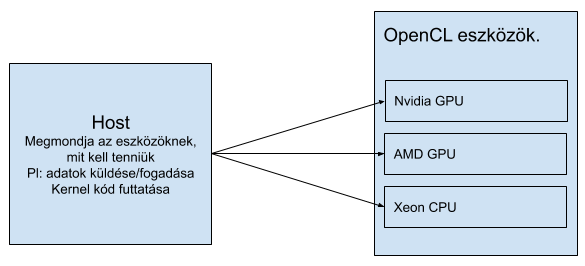
\includegraphics[width=\textwidth]{images/opencl.png}
\caption{OpenCL}
\label{fig:opencl}
\end{figure}

A következő esetekben a GPU-t érdemes használni.
\begin{itemize}
\item Gyors permutáció: Az eszközök gyorsabban mozgatáják a memóriát mint a Host.
\item Adat átváltás: Egyik formátumról másikra.
\item Numerikus gyorsítás: Az eszközök gyorsabban számolnak nagyobb adatdarabokkal mint a Host.
\end{itemize}
Jelen esetben a Host egy asztali számítógép.
Számítási eszközei: CPU, GPU, FPGA, DSP.
A számítási egységek: a magok száma
Elemek feldolgozása: ALU-k magunként.

OpenCL használata mellett szükségtelen gondolkozni azon, hogy pontosan mi is végzi el a számításokat. Ugyanis az OpenCL modelljének illeszkedése egy adott hardverhez, a gyártók feladata.


\Section{Az OpenCL telepítése}

A megfelelő működéshez az első lépést már a rendszer telepítésénél megtettem amikor a non-free avagy az nvidia eredeti drivernének a telepítését választottam.
ezen kívül a következő csomagokra volt szükség: 

\begin{python}
$ sudo pacman -S opencl-headers
$ sudo pacman -S opencl-nvidia
$ sudo pacman -S cuda
$ sudo pacman -S ocl-icd
\end{python}

\Section{Az OpenCL használata}



